\lecture{17}{Phase Transitions, van der Waals Model}{Qiang Zhu}{scribe-name1,2,3}

\section{The van der Waals Model}
To understand phase transformations more deeply, 
\begin{enumerate}
\item What's the shape of the phase boundary?
\item Why is there a critical point? What's its origin?
\end{enumerate}

we should start with a specific mathematical model.
The easiest model is perhaps to study liquid-gas transformations based van der Waals model.

In 1873, van der Waals proposed a modified model based on the ideal gas law.
\begin{equation} 
(P + \frac{a N^2}{V^2})(V-Nb) = NkT
\end{equation}

The modifications are the following,
\begin{enumerate}
\item Subtracting $Nb$ from $V$, which accounts for the minimum volume when pressure goes to infinity. 
\item Adding $aN^2/V^2$ to $P$, which accounts for the short range attractive forces.
\end{enumerate}

Why $N$ and $N^2/V^2$?\\
Considering all atoms are spheres, the minimum of $V$ must be proportional to $N$.\\
The potential energy must be proportional to its density $N \times N/V$.\\

For convenience, we can express $P$ from the vdW equation as follows
\begin{equation} 
P = \frac{NkT}{V-Nb}-\frac{aN^2}{V^2}
\end{equation}

The constants of $a$ and $b$ must be fitted for different systems.
$b$ corresponds to the molecular volume, while $a$ is much more variable because of the complex intermolecular interactions.
Now let us investigate the consequence of the vdW model.
At high $T$ regime ($V$ goes to high), it exactly behaves like gas.
At low $T$ regime, the behavior is much more complicated. As $V$ decreases the isotherm rises, falls, and then rises again.

At a given $P,T$, the true equilibrium state of a system is determined by its Gibbs free energy. To calculate $G$ for a vdW fluid, let's
start with the thermodynamic identity.
\begin{equation}
dG= -SdT + VdP + \mu dN
\end{equation}

For a fixed amount of materials, at a given temperature, this equation reduces to $dG=VdP$. Dividing both sides by $dV$ gives,
\begin{equation}
(\frac{\partial G}{\partial V})_{N,T} = V (\frac{\partial P}{\partial V})_{N,T} 
\end{equation}
The right-hand side can be computed from the vdW model,
\begin{equation}
(\frac{\partial G}{\partial V})_{N,T} = - \frac{NkTV}{(V-Nb)^2} + \frac{2aN^2}{V^2}
\end{equation}

To integrate it, we obtain
\begin{equation}
G = -NkT\text{ln}(V-Nb) + \frac{(NkT)(Nb)}{V-Nb} - \frac{2aN^2}{V} + c(T)
\end{equation}

This equation allows us to plot the Gibbs free energy for any fixed $T$.

To understand it, let's try to make the plot of $G$ as a function of $P$ and $V$. From the $G-P$ plot, we can clearly see that there is a
triangle loop in the graph (2-3-4-5-6), corresponding to the unstable states. As the pressure gradually increases, the system will go 
straight from 2 to 6, with an abrupt decrease in volume. A phase transformation therefore occurs. At point 2, we call it a gas, but point 6 a liquid.
At intermediate volumes, the thermodynamically stable state is actually a combination of part gas and part liquid, as indicated by the straight
vertical line on the $P-V$ diagram. 

The pressure at the phase transformation is easy enough to determine from the graph of $G$, but there is a way to obtain it from the $PV$ graph.
Clearly, there should be zero net work during the 2-3-4-5-6 loop, since 2, 6 are in equilibrium. This is called the {\bf Maxwell construction}.

Repeating the Maxwell construction for a variety of temperatures gives the vapor pressures. The region which the line crosses defines the regions in the coexistence of liquid and gas.
However, what will happen on high temperature? There is no way to build Maxwell construction. Hence the phase boundary must disappear at some temperature, which we call it critical temperature, $Tc$.
And the corresponding $P,V$ is called $Pc$ and $Vc$. These values defines the {\bf critical point}. If the temperature goes beyond the critical point, the liquid and gas are no longer distinguishable.
\begin{equation}
\frac{\partial P}{\partial V} = 0 ~~~~~~  \frac{\partial^2 P}{\partial V^2} = 0
\end{equation}

Prove the following relations
\begin{equation}
V_c = 3Nb ~~~~~~  P_c = \frac{1}{27} \frac{a}{b^2} ~~~~~~ kT_c = \frac{8}{27} \frac{a}{b}
\end{equation}

Homework 
Problem 5.48, 5.49, 5.51, 5.52, 5.53


\begin{figure}[h]
\centering
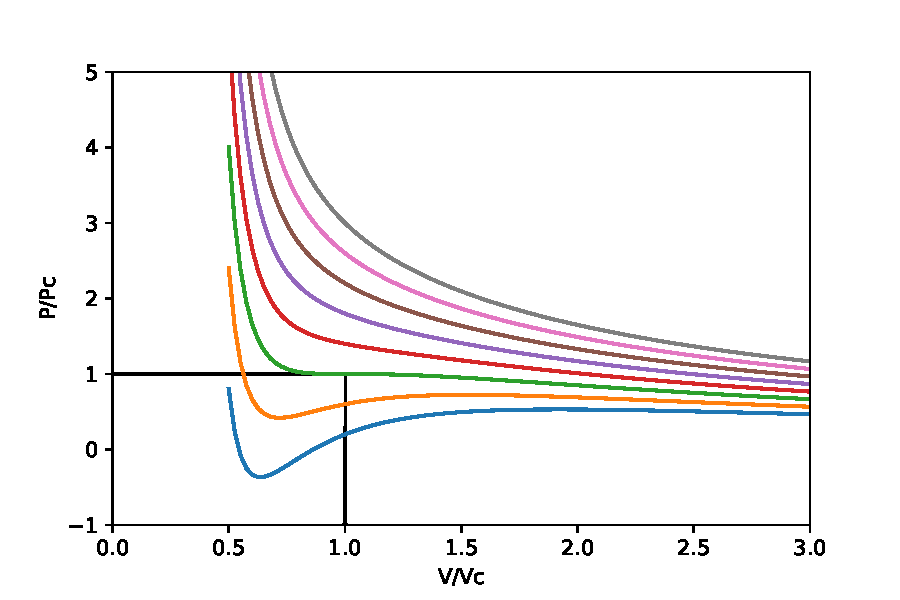
\includegraphics[width=9cm]{imgs/vdW.pdf}
\caption{$P-V$ isothermal curves close to the phase transition temperature. }
\end{figure}


\begin{figure}[h]
\centering
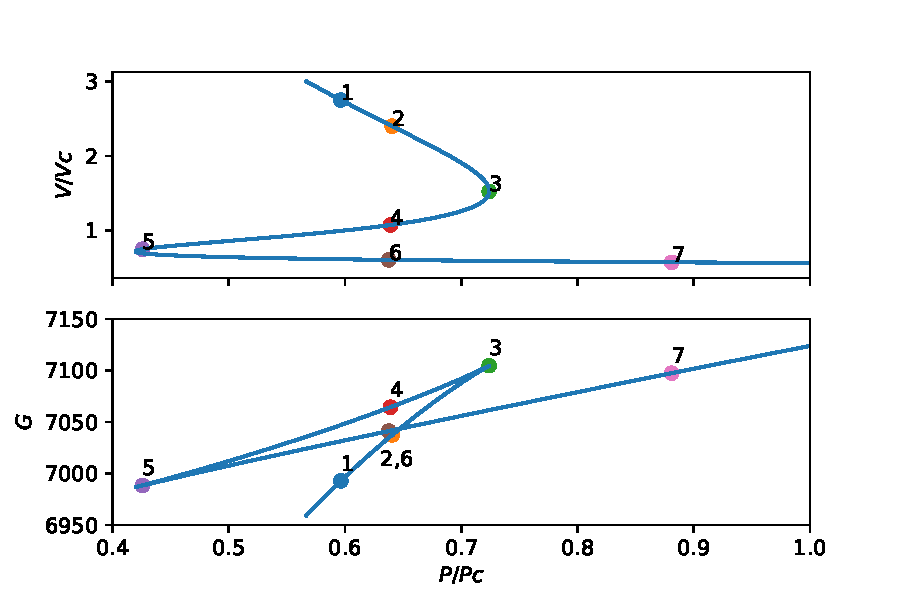
\includegraphics[width=9cm]{imgs/MaxWell.pdf}
\caption{Gibbs free energy as a function of pressure for a vdW model at $T$=0.9 Tc. The corresponding isotherm is shown at above.}
\end{figure}

\begin{figure}[h]
\centering
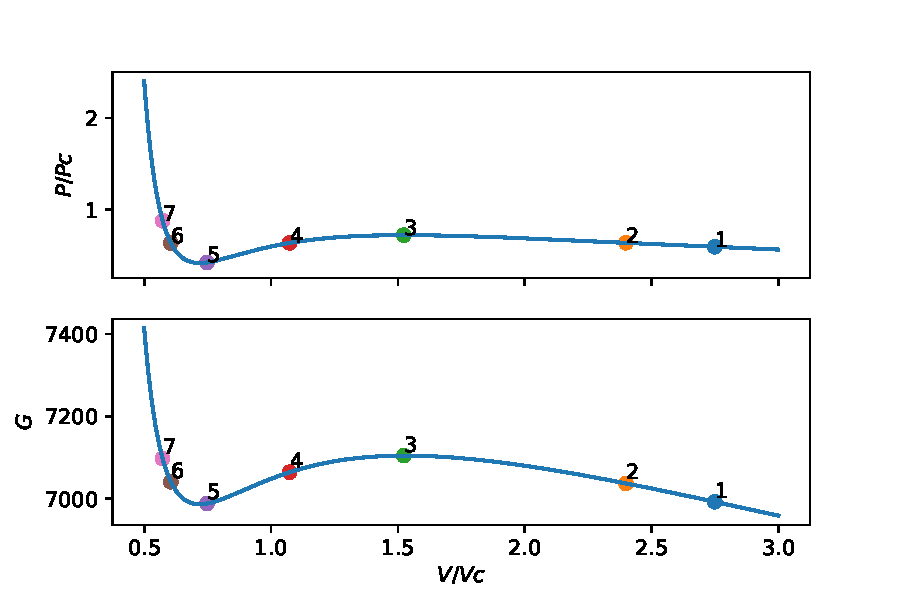
\includegraphics[width=9cm]{imgs/MaxWell-f.pdf}
\caption{Gibbs free energy as a function of volume for a vdW model at $T$=0.9 $T_c$. The corresponding isotherm is shown above.}
\end{figure}


